\section{Design Flow}

The proposed design flow is illustrated in Figure
\ref{fig:design-flow}. MaxC is used to specify dataflow
designs. Transformations specified through aspects are applied to the
original design, generating new MaxC designs. These are then compiled
by the MaxC backend to generate MaxJ design for hardware or
simulation.

The design space exploration process can be automated and ran until a
dataflow design that achieves timing closure and meets non functional
requirements is generated.  For each optimization strategy in our
repository we:

\begin{enumerate}

\item apply the set of specific low-level optimizations comprised in
  the strategy (e.g. setting DSP balance).

\item compile the optimized design using the MaxCC backend to MaxJ

\item start the backend compilation toolchain (MaxCompiler
  and Xilinx) and perform an analysis of the reporting information,
  based on which we either restart the flow with the next optimization
  strategy step or proceed to the next step

\item measure non-functional requirements such as performance or
  latency and if our target is not met we restart using a different
  optimization strategy

\end{enumerate}
\begin{comment}
  \begin{figure}[!h]
    \caption{The proposed design flow.}
    \begin{center}
      \begin{tikzpicture}[node distance = 2cm, auto, scale=0.5]
        \node [block] (csrc) {C source};
        \node [block, below of=csrc, left of=csrc] (maxrt) {CPU Runtime code};
        \node [block, below of=csrc, right of=csrc] (maxc) {MaxC Design};
        \node [block, below of=maxc] (maxj) {MaxJ Design};
        \node [block, below of=maxj] (maxfile) {Maxfile};
        \node [block, below of=maxfile, left of=maxfile] (app) {Application executable};
        \node [block, below of=app] (maxnode) {MaxNode, MaxStation};

        \node [cloud, right of=csrc] (lara) {LARA};
        \node [cloud, left of=csrc] (maxcc) {MaxCC};
        % \node [cloud, right of=init] (system) {system};
        % \node [block, below of=init] (identify) {identify candidate models};
        % \node [block, below of=identify] (evaluate) {evaluate candidate models};
        % \node [block, left of=evaluate, node distance=3cm] (update) {update model};
        % \node [decision, below of=evaluate] (decide) {is best candidate better?};
        % \node [belock, below of=decide, node distance=3cm] (stop) {stop};

        \path [line] (csrc) -- (maxrt);
        \path [line] (csrc) -- (maxc);
        \path [line] (maxc) -- (maxj);
        \path [line] (maxj) -- (maxfile);
        \path [line] (maxfile) -- (app);
        \path [line] (maxrt) -- (app);
        \path [line] (app) -- (maxnode);
        \path [line, dashed] (lara) -- (csrc);
        \path [line, dashed] (lara) -- (maxc);

        % \path [line] (decide) -| node [near start] {yes} (update);
        % \path [line] (update) |- (identify);
        % \path [line] (decide) -- node {no}(stop);
        % \path [line,dashed] (expert) -- (init);
        % \path [line,dashed] (system) -- (init);
        % \path [line,dashed] (system) |- (evaluate);
      \end{tikzpicture}
    \end{center}
  \end{figure}
\end{comment}

\begin{figure}[!h]
%  \includegraphics[scale=0.5, trim=50 180 0 50]{figs/lara_maxcc.pdf}
  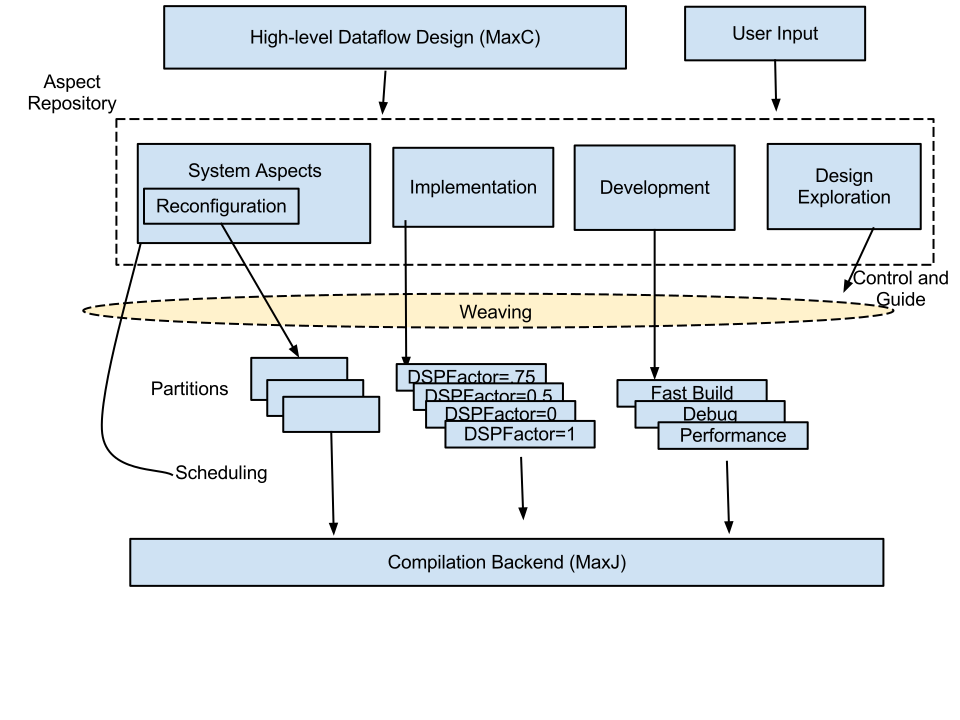
\includegraphics[scale=0.27, trim=0 0 0 0]{figs/design-flow}
  \caption{The proposed design flow.}
  \label{fig:design-flow}
\end{figure}
